\begin{figure}[htbp]
\centering
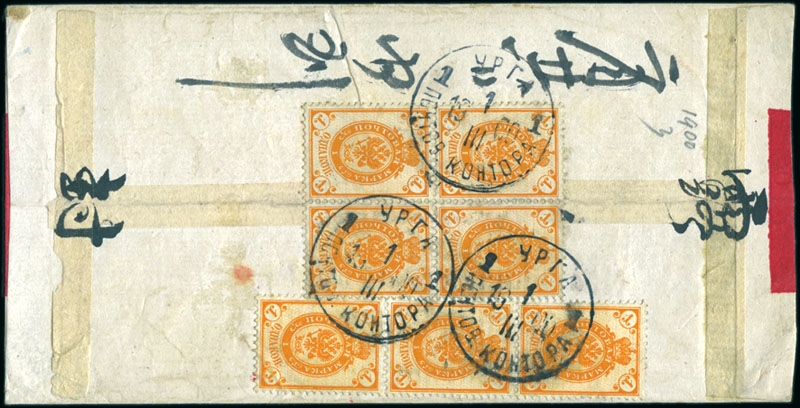
\includegraphics[width=.95\textwidth]{../russian-post-in-mongolia/10128.jpg}
\caption{ 
10128 URGA: 1900 Native cover to Kalgan, franked on the reverse with 
seven 1k orange (in strip of 3 and block of 4) paying the single rate, 
tied by crisp strikes of the Urga 1.III.1900 type 4 cds in black, fine and 
unusual franking of the 7k rate.
Provenance: Ex Tolman
\euro 400.00 
} 
\end{figure}    

\begin{figure}[htbp]
\centering
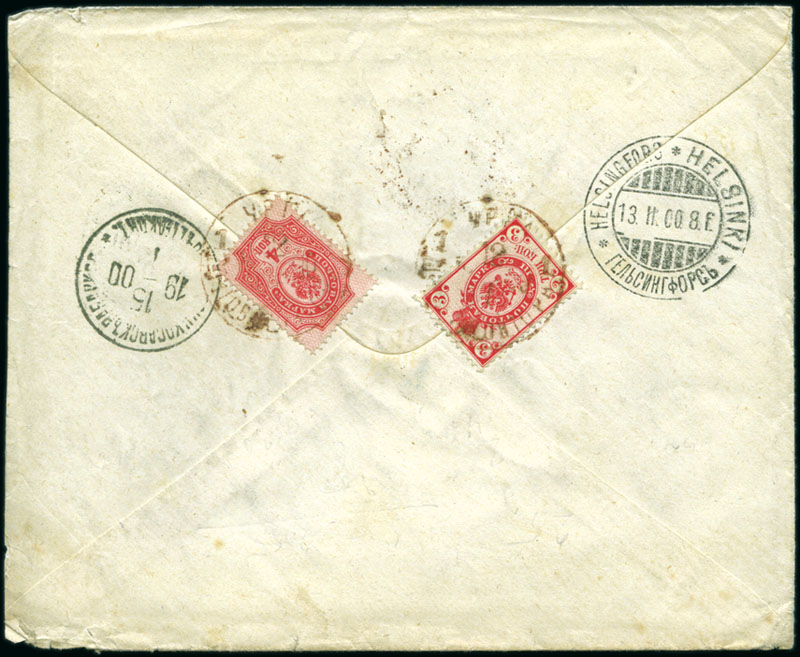
\includegraphics[width=.95\textwidth]{../russian-post-in-mongolia/10129.jpg}
\caption{ 
10129 URGA: 1900 Envelope to Helsinki (Finland), franked on the reverse with 
Russia 3k and 4k paying the singlel rate, tied by Urga 12.1.1900 type 4 cds 
in RED (rated RR by Hellrigl), with Troitskosavsk and Helsinki bs, an 
uncommon destination
\euro 300.00 
} 
\end{figure}   

\begin{figure}[htbp]
\centering
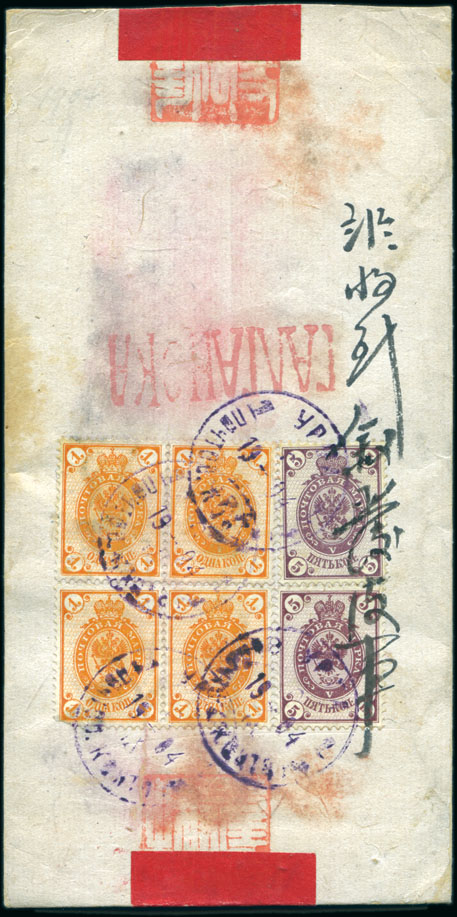
\includegraphics[width=.50\textwidth]{../russian-post-in-mongolia/10130.jpg}
\caption{ 
10130 URGA: 1904 Native cover to Kalgan, franked with two Russia Arms 5k 
and block of four 1k, paying double the rate, tied by the Urga 19.IX.04 
type 4 cds in violet, unusual franking
Provenance: Ex Tolman
\euro 400.00 
} 
\end{figure} 

\begin{figure}[htbp]
\centering
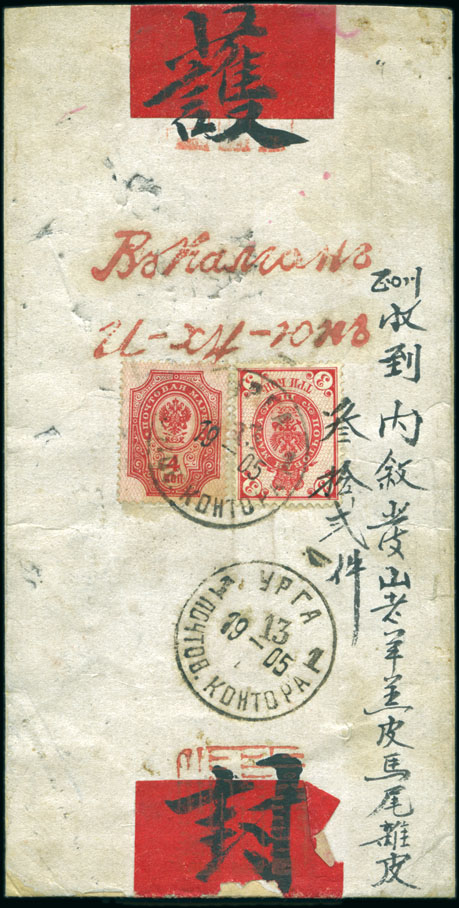
\includegraphics[width=.50\textwidth]{../russian-post-in-mongolia/10131.jpg}
\caption{ 
10131 URGA: 1905 Native cover to Kalgan, franked with 4k and 3k paying
the single rate, tied by Urga 13.I.05 type 4var cds (with "13" misplaced),
the earliest date recorded of this constant cds variety, fine.

Note: Origin of cancel illustration in "Stamps of the Russian Empire 
Used Abroad" p.316 fig.444 by Tchilinghirian \& Stephen

Provenance: Ex Tolman
\euro 200.00 
} 
\end{figure}   

\begin{figure}[htbp]
\centering
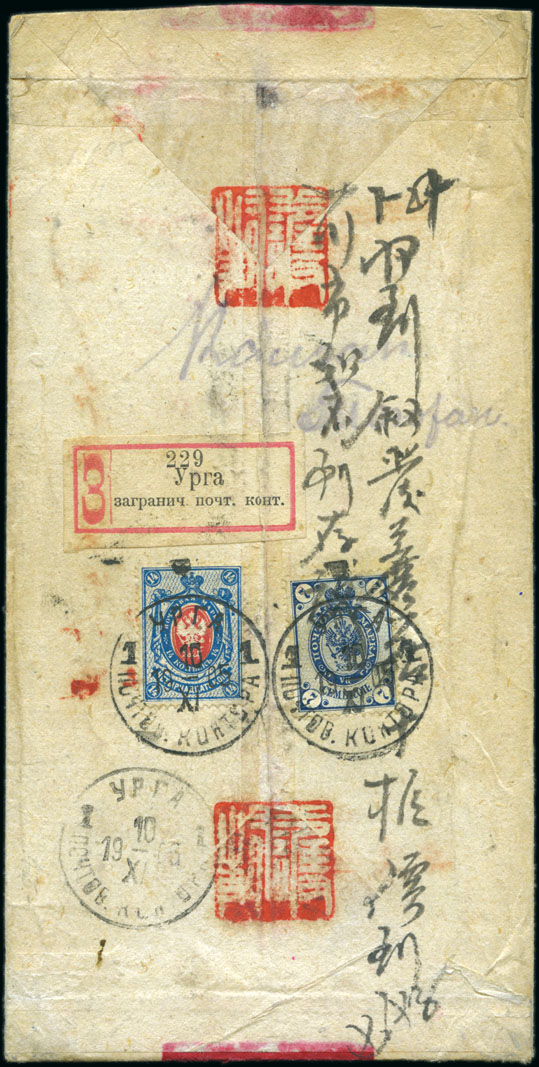
\includegraphics[width=.50\textwidth]{../russian-post-in-mongolia/10132.jpg}
\caption{ 
10132 URGA: 1905 Native cover registered to Kalgan, with Russia Arms 7k
and 14k paying double the rate plus registration fee, tied by Urga 19.XI.05
type 4 cds with registration label adjacent (Hellrigl type 4 rated RRR),
fine and rare registered cover.

Provenance: Ex Tolman
\euro 2,000.00 
} 
\end{figure}   

\begin{figure}[htbp]
\centering
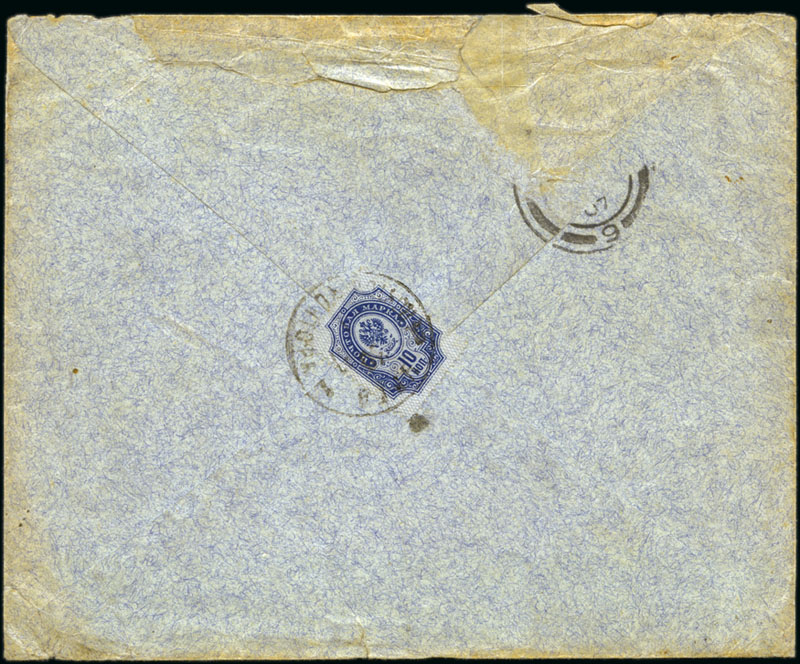
\includegraphics[width=.95\textwidth]{../russian-post-in-mongolia/10133.jpg}
\caption{ 
10133 URGA: 1907 Envelope to England with 1902-05 10k blue on the reverse 
paying the single foreign rate, tied by Urga 30.I.07 type 4 cds, small 
portion of backflap missing, otherwise a fine and very rare usage of this stamp.
\euro 300.00 
} 
\end{figure}

\begin{figure}[htbp]
\centering
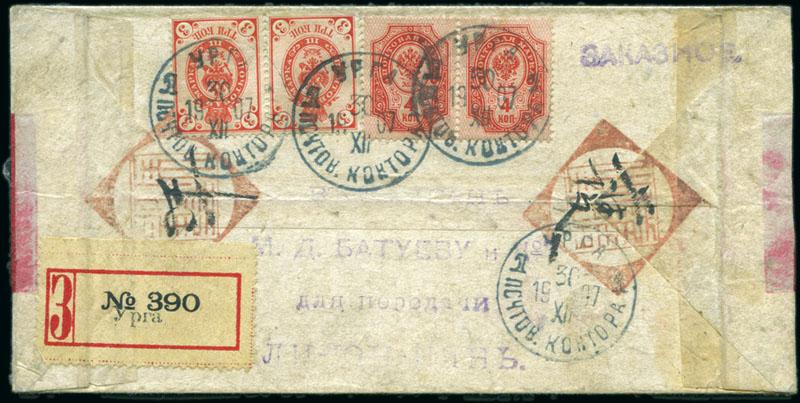
\includegraphics[width=.95\textwidth]{../russian-post-in-mongolia/10134.jpg}
\caption{ 
10134 URGA: 1907 Native cover registered to Kalgan with pair of 3k and pair of 4k
paying the single rate plus registration, tied by Urga 19.XII.07 type 4 cds
in green, registered label adjacent, fine
\euro 2,000.00
} 
\end{figure}   

\begin{figure}[htbp]
\centering
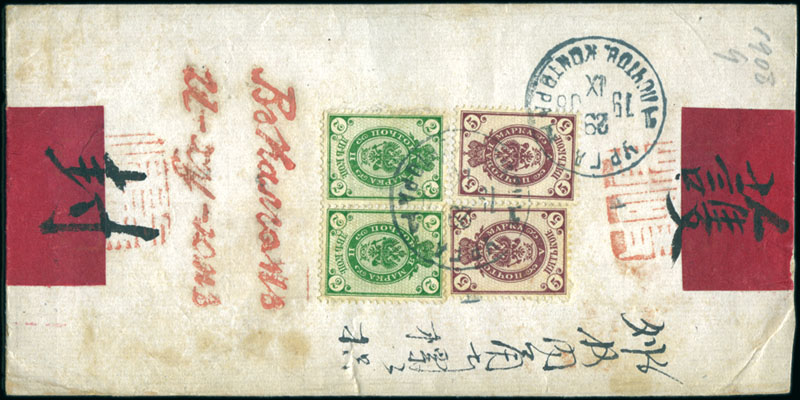
\includegraphics[width=.95\textwidth]{../russian-post-in-mongolia/10135.jpg}
\caption{ 
10135 URGA: 1908 Native cover to Kalgan, franked with two Russia Arms 2k and 
two 5k paying double the internal rate, tied by Urga 19.IX.08 type 4 cds in 
grey-black, fine

Provenance: Ex Tolman
\euro 400.00
} 
\end{figure}   

Lorem ipsum dolor sit amet, consectetur adipiscing elit. Sed nibh justo, dictum sed cursus ac, lobortis et lacus. Vestibulum vitae justo enim. Quisque laoreet elementum felis, ut sodales arcu viverra a. Sed molestie odio vulputate sem rutrum a sagittis est rutrum. Morbi dapibus hendrerit magna, sit amet commodo massa posuere sit amet. Duis pharetra quam scelerisque est lobortis fringilla. Maecenas venenatis feugiat lectus, vel facilisis odio pharetra quis. Etiam at nisl eros, sit amet suscipit lorem. Lorem ipsum dolor sit amet, consectetur adipiscing elit. Sed augue nunc, ornare eget congue sit amet, laoreet vel augue. Morbi vel justo quis ipsum adipiscing egestas vitae non est. Vivamus ac quam quam. Nullam pharetra
                                                    interdum mauris, rutrum pulvinar ligula condimentum id. Donec et blandit lorem. 

\begin{figure}[htbp]
\centering
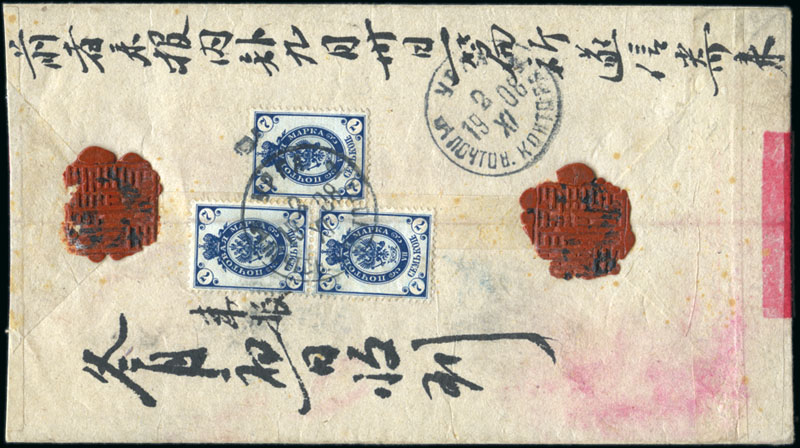
\includegraphics[width=.95\textwidth]{../russian-post-in-mongolia/10136.jpg}
\caption{ 
10136 URGA: 1908 Native cover to Kalgan, with three Russia Arms 7k paying 
triple the rate, tied by Urga 2.XI.08 type 4 cds, attractive private wax 
seal alongside.

Provenance: Ex Tolman
\euro 300.00
} 
\end{figure}   

\begin{figure}[htbp]
\centering
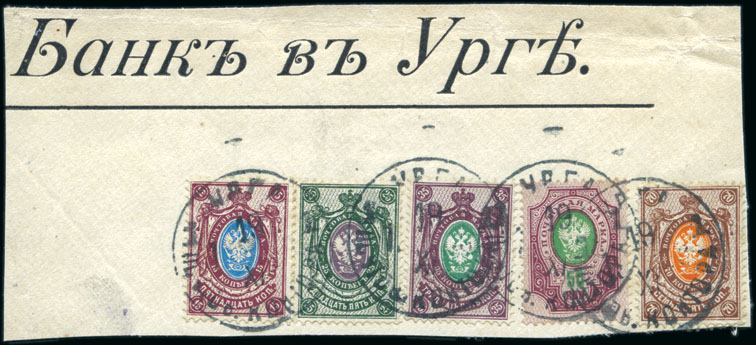
\includegraphics[width=.95\textwidth]{../russian-post-in-mongolia/10137.jpg}
\caption{ 
10137 URGA: Selection of nine stamps with the Urga type 4 cds, incl. piece 
with 1902-05 15k, 25k, 35k, 50k and 70k, plus singles of the 7r (one with 
black cds, one with violet cds) and 10R (one with grey-black, one with black cds),
mainly fine
\euro200.00
} 
\end{figure}   





      